\section{Zadání}

Seznamte se s jádrem datového modelu IS STAG a vytvořte v nástroji Oracle Data Integrator Studio integrační projekt.
Předpokládá se, že výsledný projekt bude integrovat data do výsledného modelu obsahující minimálně dvě tabulky v relaci 1:N.
Bylo by též vhodné, aby nad jednou z těchto tabulek byla provedena vhodná selekce a druhá tabulka získala novou hodnotu za pomoci agregované funkce.

Téma: Průměrné hodnocení Diplomových prací z kateder FAV,

\begin{itemize}
    \item filtrace: katedry FAV (dimenzionální tabulka);
    \item agregace: průměrné hodnocení DP z kateder (faktová tabulka agregovaná přes obory).
\end{itemize}

\section{Osnova}

\begin{itemize}
    \item LM: Tabulky obory, abn\_diplomove\_prace, cis\_pracovist
    \item LM: analýza: Co obsahují, relevantní sloupce a jejich datové typy, další související tabulky (mimo rozsah zadání), vazby, exportovaný obrázek schématu
    \item L: Vypracování
    \item L: Postup tvorby
    \item L: založili jsme 2 Datové zdroje (in/out), založení tabulek ve výstupním datovém zdroji + skript, fyzické schéma, kontext, logické schéma, + tabulka z rekapitulace na \nolinkurl{https://www.kiv.zcu.cz/studies/predmety/ins/odi-topology.html})
    \item L: Datové modely (máme 2, pro každou výstupní tabulku), vazba dat
    \item M: popis transformace (agregace a filtrace). + obrázky obou mapování (Projects -> Mappings), podmínky filtrů, agregací a joinů.
\end{itemize}

Samotnému vytvoření komponent ETL předcházelo založení hlavního (MASTER\_INS\_REPO) a pracovního repozitáře (TAUCHENL\_REPO).

Nepotřebné sloupce je možné z tabulek odebrat v nabídce Designer -> Models -> <Model folder> -> <Model> -> <Tabulka> (pravý klik) -> Open -> Attributes.
Po výběru nepotřebných atributů je možné pomocí tlačítka Delete Attribute sloupce z modelu odstranit.

\subsection{Zakládací skript}

\begin{lstlisting}[language=sql]
CREATE TABLE TRG_KATEDRY (
  KATEDRA_ID NUMERIC(16),
  KATEDRA_KOD VARCHAR(50) NOT NULL,
  KATEDRA_NAZEV VARCHAR(100),

  CONSTRAINT PK_TRG_KATEDRY PRIMARY KEY (KATEDRA_KOD)
);

CREATE TABLE TRG_HODNOCENI_DP (
  KATEDRA_KOD VARCHAR(50),
  OBOR_ID NUMERIC(10) NOT NULL,
  OBOR_NAZEV VARCHAR(55),
  HODNOCENI VARCHAR(50),

  CONSTRAINT PK_TRG_HODNOCENI_DP PRIMARY KEY (OBOR_ID),
  CONSTRAINT FK_KATEDRY_HONOCENI FOREIGN KEY (KATEDRA_KOD) REFERENCES TRG_KATEDRY (KATEDRA_KOD)
);
\end{lstlisting}

\section{Vypracování}

\begin{figure}[htb]
    \centering
    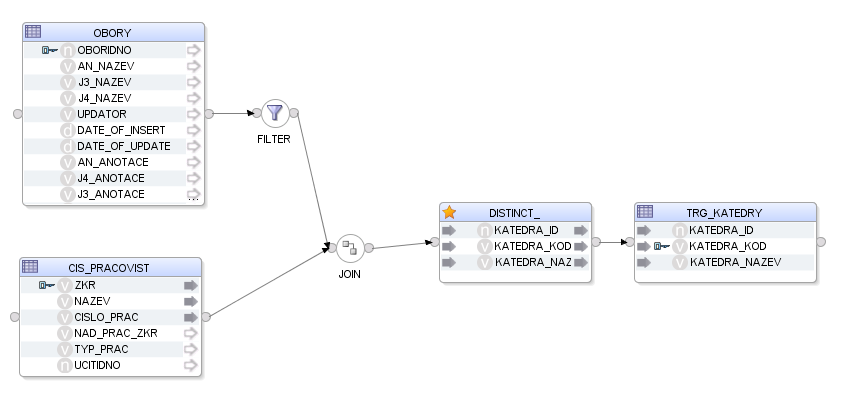
\includegraphics[width=0.7\textwidth]{graphs/odi-mapping-trg-katedry.png}
    \caption{ODI Výstupní mapování do tabulky TRG\_KATEDRY, logické schéma}
    \label{fig:odi-mapping-trg-katedry}
\end{figure}
\FloatBarrier

\begin{figure}[htb]
    \centering
    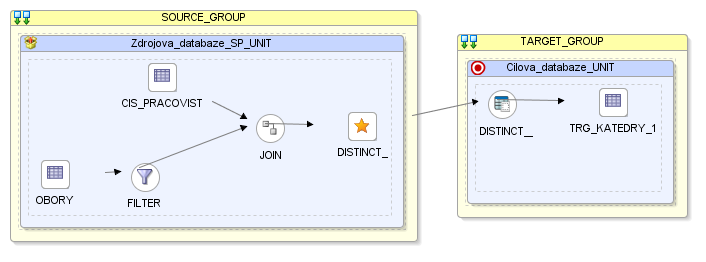
\includegraphics[width=0.7\textwidth]{graphs/odi-mapping-trg-katedry-physical.png}
    \caption{ODI Výstupní mapování do tabulky TRG\_KATEDRY, fyzické schéma}
    \label{fig:odi-mapping-trg-katedry-physical}
\end{figure}
\FloatBarrier

\begin{figure}[htb]
    \centering
    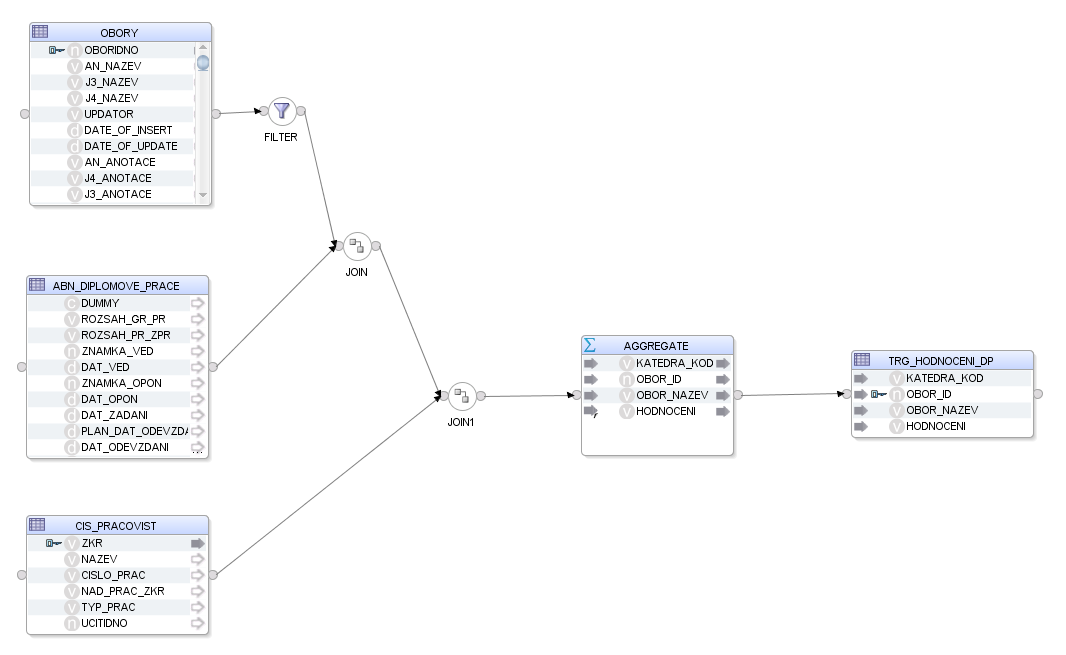
\includegraphics[width=0.7\textwidth]{graphs/odi-mapping-trg-hodnoceni-dp.png}
    \caption{ODI Výstupní mapování do tabulky TRG\_HODNOCENI\_DP, logické schéma}
    \label{fig:odi-mapping-trg-hodnoceni}
\end{figure}
\FloatBarrier

\begin{figure}[htb]
    \centering
    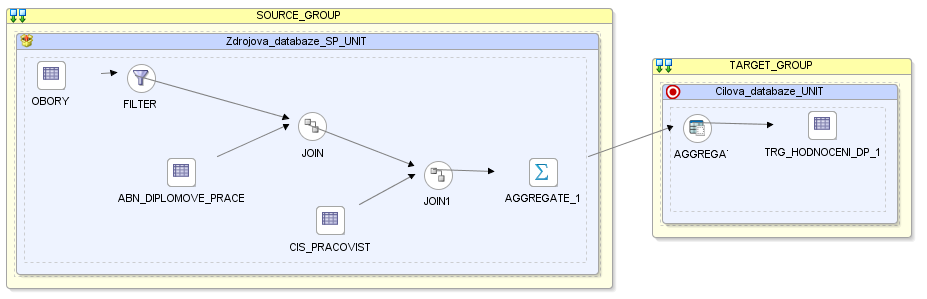
\includegraphics[width=0.7\textwidth]{graphs/odi-mapping-trg-hodnoceni-dp-physical.png}
    \caption{ODI Výstupní mapování do tabulky TRG\_HODNOCENI\_DP, fyzické schéma}
    \label{fig:odi-mapping-trg-hodnoceni-physical}
\end{figure}
\FloatBarrier

\begin{figure}[htb]
    \centering
    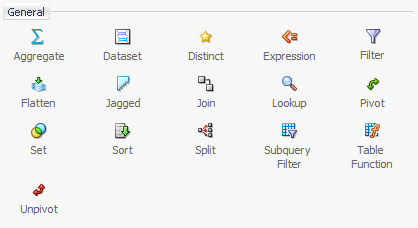
\includegraphics[width=0.55\textwidth]{graphs/odi-transformation-components.png}
    \caption{ODI nabídka komponent}
    \label{fig:odi-transformation-components}
\end{figure}
\FloatBarrier

\begin{figure}[htb]
    \centering
    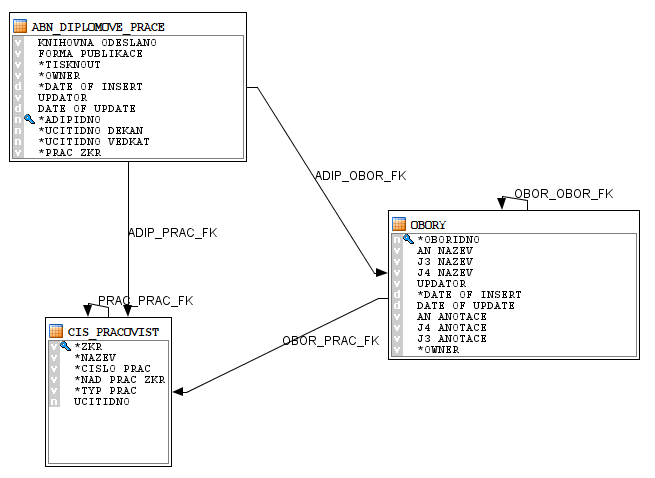
\includegraphics[width=0.3\textwidth]{graphs/src-model.png}
    \caption{Vstupní model}
    \label{fig:src-model}
\end{figure}
\FloatBarrier

\subsection{Výstupní model \& data}

Model výstupních dat je znázorněn na obrázku~\ref{fig:trg-model}.
Myšlenka tohoto schéma je poskytnout dimenzionální pohled na data, s tabulkou \textit{TRG\_KATEDRY} jako dimenzí a \textit{TRG\_HODNOCENI\_DP} jako faktovou tabulkou.

\begin{figure}[htb]
    \centering
    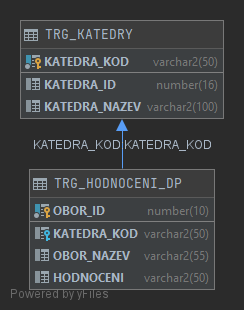
\includegraphics[width=0.3\textwidth]{graphs/trg-model.png}
    \caption{Výstupní model}
    \label{fig:trg-model}
\end{figure}
\FloatBarrier

Výstupní data z transformací jsou k vidění v tabulkách~\ref{table:table1}~\&~\ref{table:table2}.
Jak již vyplývá z předešlého popisu, tabulka \textit{Katedry} obsahuje 3 sloupce: \textit{KATEDRA\_ID}, \textit{KATEDRA\_KOD} a \textit{KATEDRA\_NAZEV}.

\textit{KATEDRA\_ID} měl původně sloužit jako primární klíč celé tabulky, z důvodu praktičnosti byl však v účelu nahrazen jejím kódem.
Tabulka obsahuje, dle zadání, pouze katedry FAV.

\begin{table}[htb]
    \centering

    \begin{tabular}{lll}
        \toprule

        KATEDRA\_ID & KATEDRA\_KOD  & KATEDRA\_NAZEV                            \\ \midrule
        52110       & KFY           & Katedra fyziky                            \\
        52120       & KME           & Katedra mechaniky                         \\
        52130       & KMA           & Katedra matematiky                        \\
        52140       & KKY           & Katedra kybernetiky                       \\
        52150       & KIV           & Katedra informatiky a výpočetní techniky  \\
        52160       & KGM           & Katedra geomatiky                         \\
          
        \bottomrule
    \end{tabular}

    \caption{Data ve výstupní tabulce TRG\_KATEDRY}
    \label{table:table1}
\end{table}
\FloatBarrier

Faktová tabulka \textit{Hodnocení} obsahuje 4 sloupce: \textit{KATEDRA\_KOD}, \textit{OBOR\_ID}, \textit{OBOR\_NAZEV} a~\textit{HODNOCENI}.
Abychom docílili splnění zadání, hodnocení je agregát (průměrná hodnota) hodnocení pro každý z oborů referencovaných kateder.
Jelikož by každý obor měl být v tabulce pouze jednou, je identifikační číslo oboru použito jako primární klíč.

\begin{table}[htb]
    \centering

    \begin{tabular}{llll}
        \toprule

        KATEDRA\_KOD    & OBOR\_ID  & OBOR\_NAZEV                       & HODNOCENI \\ \midrule
        KIV             & 2252      & Softwarové inženýrství            & 2,25      \\
        KGM             & 2309      & Geomatika                         & 4         \\
        KGM             & 2358      & Geomatika                         & 1,875     \\
        KKY             & 3808      & Automatické řízení a robotika     & NULL      \\
        KMA             & 2130      & Finanční informatika a statistika & 2,6667    \\
        \ldots          & \ldots    & \ldots                            & \ldots    \\

        \bottomrule
    \end{tabular}

    \caption{Ukázková data z výstupní tabulky TRG\_HODNOCENI\_DP}
    \label{table:table2}
\end{table}
\FloatBarrier

\section{Závěr}

V semestrální práci jsme si vyzkoušeli proces vytváření datové transformace.
Tento proces byl náplní praktických cvičení, jednalo se tedy hlavně o důkaz replikovatelnosti postupu na vlastním zadání.
Použitý nástroj, Oracle Data Integrator, je jeden z nejrozšířenějších ETL produktů vůbec.

Praktická cvičení a semestrální práce nám tedy poskytli cennou příležitost zkusit si s tímto nástrojem pracovat a řešit případné potíže, které mohou při konstrukci transformací nastat.
V našem konkrétním případě se pak jedná i o zajímavé propojení předmětů, jelikož jsme zvolili transformaci z logického databázového modelu do dimenzionální struktury, poskytujíc referenci na předmět KIV/DBM2.

Jelikož nástroj ODI není jediným produktem tohoto zaměření, stojí za to zmínit silné a slabé stránky produktu.
Společnost Oracle je velmi silný dodavatel, poskytující robustní podporu svých produktů, a to zejména v případech tak ověřených nástrojů jakým je Data Integrator.
Na druhou stranu nelze opomenout zastaralé uživatelské rozhraní, strmou křivku učení a v našich podmínkách velmi pomalé chování.

Za zmínku stojí také možnost nahlédnutí do databáze demo verze systému IS STAG, která přes přítomnost pouze testovacích dat poskytuje bohaté datové schéma k prozkoumání.
